% Metódy inžinierskej práce

\documentclass[10pt,slovak,a4paper]{article}

\usepackage[slovak]{babel}
%\usepackage[T1]{fontenc}
\usepackage[IL2]{fontenc} % lepšia sadzba písmena Ľ než v T1
\usepackage[utf8]{inputenc}
\usepackage{graphicx}
\usepackage{url} % príkaz \url na formátovanie URL
\usepackage{hyperref} % odkazy v texte budú aktívne (pri niektorých triedach dokumentov spôsobuje posun textu)
\usepackage{float}

\usepackage{cite}
%\usepackage{times}

\pagestyle{headings}

\title{Vývoj softvérových projektov v rámci Scrum\thanks{Semestrálny projekt v predmete Metódy inžinierskej práce, ak. rok 2020/21, vedenie: Ing. Vladimír Mlynarovič, PhD}}
\author{Michal Darovec\\[2pt]
	{\small Slovenská technická univerzita v Bratislave}\\
	{\small Fakulta informatiky a informačných technológií}\\
	{\small \texttt{xdarovec@stuba.sk}}
	}

\date{\small 26. október 2021}



\begin{document}

\maketitle

\begin{abstract}
Cieľom tejto práce je predstaviť a bližšie ukázať spôsob vývoja softvérových projektov v rámci Scrum. V práci sa zoznámime s agilnou metodikou, v ktorej sa v súčasnosti robí veľké množstvo nielen softvérových projektov. Ďalej sa v práci zameriame priamo na Scrum, predstavíme si jeho princípy, pravidlá a filozofiu. Čitateľ bude oboznámený s problematikou Scrumu, rovnako s jeho výhodami a nevýhodami.

\textbf{Kľúčové slová:} agile, scrum, softvérový projekt, vývoj, inžinierstvo
\end{abstract}



\section{Úvod}

Agilná metodika je stále viac populárny spôsob vyvíjania softvérových projektov a väčšina efektívnych firiem ju v tejto dobe využíva. Ide o skupinu frameworkov, ktoré fungujú na princípe iteratívneho vývoja a na kolaborácii samostatne pracujúcich funkčných tímov.
Celá filozofia agilnej metodiky je zameraná na inováciu. Ľudia v dnešnej dobe pracujú vo vysoko dynamických prostrediach, kde inovácia je nevyhnutne potrebná pre úspešný vývoj produktu. Moderné technológie sa vyvíjajú tak rýchlo, že ak firma neaplikuje dynamický prístup, produkty môžu byť zastarané a prakticky nepoužiteľné.

Najznámejší framework agilnej metodiky je Scrum. Jeho cieľom je pomôcť ľuďom, tímom a organizáciám vytvárať hodnotu prostredníctvom prispôsobivého riešenia komplexných problémov. Scrum nie je detailne špecifikovaný, jeho pravidlá sú skôr na správne nasmerovanie a udržiavanie disciplíny v podniku. Ako uvádzajú hlavní vývojári tohto frameworku, Ken Schwaber a Jeff Sutherland: „Scrum je postavený na kolektívnej inteligencii ľudí, ktorí ho používajú.“~\cite{schwaber2020scrum}. K jeho hodnotám a filozofii sa dostaneme bližšie v časti~\ref{hodnoty}.

Scrum je hlavne založený na princípe rýchleho a efektívneho vývoja produktov, ktorý je v dnešnej dynamickej dobe kľúčový. Tieto dynamické princípy môžeme vidieť hlavne v svetových softvérových firmách. Scrum však nie je výhodné implementovať pri veľkom množstve rutinných a repetitívnych úloh, ako napríklad pri účtovníctve alebo predajných hovoroch.~\cite{agile} Aj keď s prechodom na Scrum prichádza veľké riziko, osvojuje si ho viac a viac progresívnych manažérov. Začína sa dokonca stále viac používať mimo sféry softvérového inžinierstva.

\section{Hodnoty a filozofia} \label{hodnoty}

Skôr, ako sa pustíme do jednotlivých častí tohto frameworku, ideme si opísať, na čom je Scrum vlastne postavený. Tvorcovia Scrumu sa inšpirovali empiristickou filozofiou, ktorej základné myšlienky sú, že vedomosti nadobúdame zo skúseností a rozhodnutia robíme na základe toho, čo máme preskúmané. Scrum je postavený aj na "lean thinking", čo je metóda organizovania ľudských aktivít takým spôsobom, aby sa ľudia nemrhali časom a sústredili sa na to najdôležitejšie~\cite{schwaber2020scrum}. Už z filozofie môžeme pochopiť, na akých princípoch Scrum funguje. Jedná sa o framework, v ktorom sa ľudia učia z vlastných chýb a sústredia sa na to najdôležitejšie, aby nestrácali čas na nepodstatných veciach. Takáto filozofia podnecuje produktivitu a dynamickosť vývojárov.

Pre správne fungovanie Scrumu je potrebné, aby bol celý tím zdatný týchto v piatich oblastiach: \emph{oddanosť, zameranie sa, otvorenosť, rešpekt a odvaha}. Scrum Tím musí byť oddaný splniť všetky svoje úlohy. Prvoradé zameranie Scrum Tímu je šprint, pri ktorom chce vždy spraviť čo najväčší progres. Viac o šprinte si povieme neskôr. Pri práci v tíme je vždy dôležité vzájomne sa rešpektovať. Ľudia v Scrum Tíme sú otvorení, hlavne čo sa týka vecí, na ktorých spoločne pracujú. Nevyhýbajú sa ťažkým problémom, majú odvahu im čeliť a riešiť ich~\cite{schwaber2020scrum}. Tieto hodnoty by mali byť základnou mentalitou všetkých Scrum Tímov. V dynamických prostrediach je z hľadiska maximálnej produktivity nutné ich dodržiavať, aby bol tím čo najefektívnejší a využíval plný potenciál Scrumu. 

\section{Funkcie v Scrume} \label{funkcie}

Scrum dodržiava špecifický spôsob rozdeľovania úloh pri vývoji projektov. Scrum Tím je tím všetkých účastníkov v Scrum procese, ktorý sa rozdeľuje na Scrum Mastera, Product Ownera a samotný Tím, teda tím developerov. Treba rozlišovať Tím a Scrum Tím, tieto pojmy sa často mýlia. Všetci účastníci Scrumu spolu blízko spolupracujú, komunikujú a riešia problémy. Snažia sa sústrediť sa vždy na jeden spoločný cieľ, ktorý sa v Scrume nazýva Product Goal. Scrum Tímy prirodzene fungujú lepšie, keď sú menšie, ľudia spolu vedia bližšie komunikovať a sú produktívnejší. Menej ľudí tak často spraví viac práce. Ukázalo sa, že najvýhodnejšie je mať v tíme 10 a menej ľudí. Vo veľkých spoločnostiach preto treba Scrum správne implementovať, čo vyžaduje skúsených manažérov.

\subsection{Scrum Master} \label{funkcie:master}

Scrum Master je hlavný dozorca všetkých projektov, dáva pozor, aby všetky procesy prebiehali tak, ako majú. Jeho hlavnou úlohou je zaistiť, aby bol tím čo najproduktívnejší a aby čo najrýchlejšie splnil požadovaný cieľ.~\cite{cprime} Mal by byť pohotový a vedieť narýchlo organizovať stretnutia tímu. Rola Scrum Mastera je veľmi zložitá, vyžaduje veľkú zodpovednosť a množstvo skúseností. 
Jeho zodpovednosťou je:

\begin{itemize}
\item naučiť Product Ownera, ako dosiahnuť čo najväčší zisk na investícii
\item zvýšiť produktivitu Tímu vývojárov v každom možnom ohľade
\item robiť pravidelné záznamy najnovšieho progresu v projekte tak, aby boli dodstupné pre každého
\item pomáhať vývojárom rozvíjať kreativitu a sebavedomie
\item zlepšovať technické postupy a pomôcky, aby boli všetky funkcionality aktuálne a použiteľné~\cite{cprime}
\end{itemize}

Keď je niekto Scrum Master, nestačí, že má dobré manažérske schopnosti, musí byť aj úplne stotožnený s fungovaním Scrumu, rozumieť technickým úlohám vývojárov, aby ich vedel v prípade potreby usmerniť a pomôcť im. Mal by vedieť vytvoriť prostredie, v ktorom ľudia vedia efektívne komunikovať a vzájomne si pomáhať s problémami. Keď vývojári pracujú na projekte, Scrum Master má vždy prehľad o aktuálnom stave projektu, zabezpečuje, aby sa postupovalo čo najrýchlejšie a v prípade prekážok, ktoré brzdia postupovanie projektu, ich okamžite skúša odstrániť.~\cite{cprime} Je maximálne flexibilný a má rozvinuté schopnosti riešenia problémov. Zdalo by sa, že keď má takéto zodpovednosti, tak zadáva Tímu úlohy, ale zadávanie úloh je práca Tímu. Je však jeho úlohou akokoľvek Tím povzbudiť a zjednodušiť mu rozhodovanie a riešenie problémov. Mal by vedieť naučiť svoj Tím správne a samostatne sa rozhodovať a vedieť sa navzájom dohodnúť.~\cite{cprime}


\subsection{Product Owner} \label{funkcie:owner}

Product Owner, alebo vlastník výrobku má za úlohu ukladať všetky požiadavky. Robí zástupcu zákazníkom a všetkým, ktorí sú nejakým spôsobom začlenení v projekte, takzvaným~\emph{stakeholders}. Čo sa týka požiadaviek a plánov, Tím má za úlohu počúvať iba Product Ownera. Jeho slovo je v projekte dôležité, ale táto funkcia so sebou nesie veľa rizík. Product Owner totiž nesie zodpovednosť za výrobok, rovnako ako za návrat investície na produkte. Musí sa preto snažiť o čo najväčšie zisky v porovnaní s nákladmi na výrobu výrobku. Tým, že úloha Product Ownera môže byť pri niektorých projektoch veľmi náročná, môže mať aj svoj vlastný tím, okrem Tímu vývojárov. Jeho úlohou je blízko spolupracovať s Tímom vývojárov a čo najjednoduchšie mu vysvetliť požiadavky používateľov a rôzne iné technické problémy. Mal by vedieť sprostredkovať Tímu, čo presne sa od nich chce v rámci vývoja produktu. ~\cite{techScrum}. Tiež má na starosti postup vývoja, ktoré veci implementovať skôr a ktoré naopak neskôr. Okrem týchto zodpovedností má za úlohu udržiavať~\emph{Product Backlog}, teda úložisko všetkých informácií o produkte. Toto úložisko musí pravidelne aktualizovať, aby tvoril aktuálny zoznam požiadaviek pre Tím vývojárov, aby vedeli, čo sa od nich očakáva, akým spôsobom majú vyvíjať produkt a akým veciam sa pri vývoji vyhýbať.~\cite{cprime}

\subsection{Scrum Tím} \label{funkcie:tim}

Tím developerov je v softvérových firmách samostatne fungujúci, krížovo funkčný tím vývojárov, ktorí spolupracujú na vývoji a testovaní produktu. V porovnaní s inými pracovnými štruktúrami je Tím v Scrume do veľkej miery samostatný, má autoritu robiť vlastné rozhodnutia o postupe svojej práce.~\cite{cprime} 

Samostatne sa organizujúci tím má veľa výhod, nie je závislý na manažérovi a vie si prácu lepšie rozdeliť. Členovia Tímu sa vždy najskôr spoločne dohodnú, ako postupovať pri robení úloh, ako ich rozdeliť na menšie časti a spolu s tým rozhodujú, kto bude robiť na akej časti. Čo sa týka veľkosti Tímu, ako už bolo spomenuté, Tím funguje lepšie, keď má menej účastníkov, ideálny počet je teda od troch po desiatich ľudí. Keby mal Tím viac ľudí, už by začínali byť problémy s komunikáciou, viac ľudí by sa ťažšie dohodlo na rozdelení úloh a spôsobe robenia projektu.~\cite{cprime}

Členovia Tímu sú zodpovední aj za:
\begin{itemize}
\item sledovanie stavu projektu počas Šprintu
\item vytvorenie plánu pre Šprint, tzv. Sprint Backlog
\item pravidelné aktualizovanie plánu až po dosiahnutie cieľa
\item ostatných členov Tímu a ich prácu~\cite{schwaber2020scrum}
\end{itemize}

\section{Vývojový Proces} \label{proces} 

Vývojový proces sa skladá zo Šprintu a niekoľkých porád, pri ktorých sa na Šprint pripravuje alebo sa vyhodnocujú jeho výsledky. Porady sú najlepšia príležitosť implementovať prvky Scrumu a oboznámiť s nimi ľudí, ktorí ich tak dobre nepoznajú. Vývojový proces nie je komplikovaný, skladá sa z vytvorenia Product Backlogu, úložiska všetkých informácií a požiadaviek o produkte, plánovania Šprintu, vytvorenia Sprint Backlogu a zo samotného Šprintu. Po ukončení tohto procesu máme vytvorený potenciálne odovzdateľný produkt, v Scrume ho označujeme ako inkrement. Celý vývojový proces trvá 2 až 4 týždne a opakuje sa dovtedy, kým nie je vytvorený produkt podľa požiadaviek.~\cite{techScrum} 

\begin {figure} [H]
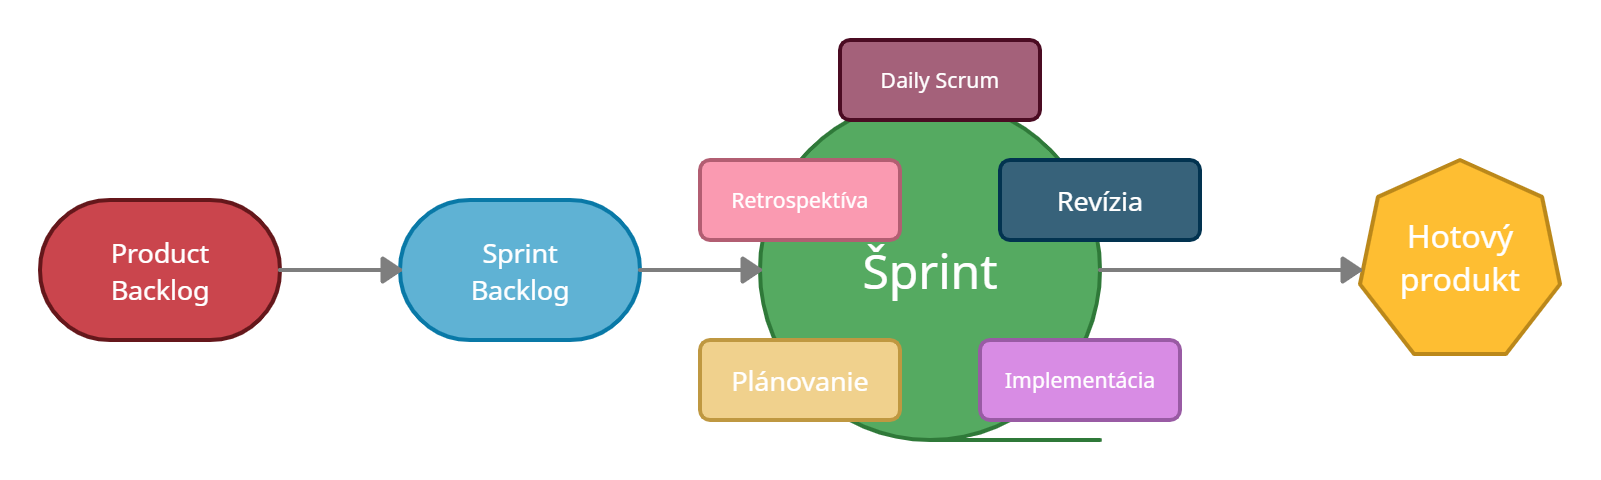
\includegraphics[scale=0.22]{diagram.png} 
\caption{Vývojový proces v Scrume\cite{wrike}}
\label{fig1}
\end {figure}

\subsection{Šprint}

Šprint je základný stavebný kameň Scrumu. Je to fáza, v ktorej sa vytvorí celý produkt od začiatku až do konca. Tu sa myšlienky a nápady menia na výsledky projektov. Šprinty sa opakujú toľkokrát, koľko je potrebné na splnenie ~\emph{Product Goal}, teda kým nie je vytvorený hotový produkt so všetkými potrebnými vylepšeniami. ~\cite{schwaber2020scrum}
Pri Šprinte by sme sa mali riadiť základnými pravidlami Scrumu, ktoré sú nastavené tak, aby sme sa vyhli neproduktivite a stagnácii. Po prvé, nerobia sa žiadne zmeny, ktoré by mali ohroziť Sprint Goal. Celý projekt by sa takto dostal do ohrozenia a v prípade neúspechu tohto plánu by sa muselo začať veľa vecí vyvíjať odzačiatku. V softvérových projektoch je to obzvlášť dôležité, lebo jednotlivé časti projektu spolu veľakrát blízko súvisia. Ďalšie pravidlo je, že kvalita sa nikdy neznižuje. Môžeme robiť zmeny, ale nikdy nie na úkor kvality vývoja. Product Owner spolupracuje s Tímom a môžu sa robiť zmeny v Product Backlogu, teda v požiadavkách na produkt. ~\cite{schwaber2020scrum}
Podľa potreby je výhodné prispôsobiť si dĺžku jedného Šprintu pre čo najefektívnejší vývoj. Cez dlhý Šprint toho Tím stihne viac a je jednoduchšie dosiahnuť prirodzený flow. Má to však aj nevýhody, lebo ak je Šprint príliš komplexný, Tím sa môže zaseknúť a projekt je v ohrození. Kratšie projekty majú výhodu, že je projekt vystavený menšiemu riziku a Tím vývojárov má jednoduchšie a jasnejšie ciele. Preto je ideálny čas trvania 1 až 4 týždne. Softvérové tímy si teda môžu vybrať trvanie, ktoré im vyhovuje najviac. O jednotlivých cykloch môžeme premýšľať ako o malých projektoch, ktoré sa nabaľujú jeden na druhý. Pri nedosiahnutí cieľu sa Šprint môže aj zrušiť, ale na to má autoritu iba Product Owner, keďže zodpovedá za celý projekt. ~\cite{schwaber2020scrum}


\subsection{Plánovanie}

Šprint je najdôležitejšia časť vývojového procesu, musí tak byť správne naplánovaný. Tento plán je zostavený kolektívnou prácou celého Scrum Tímu. Product Owner tu zohráva veľkú úlohu, lebo Product Backlog, teda súhrn požiadaviek na produkt, určuje, aké vylepšenia treba implementovať a ako dosiahnuť cieľ produktu, Product Goal. Celý Scrum Tím teda debatuje o tom, akým spôsobom sa bude postupovať v Šprinte a ako splnia Sprint Goal a s tým aj čo najviac požiadaviek z Product Backlogu. Toto plánovanie trvá maximálne 8 hodín pre jeden mesačný Šprint, nikdy nie viac. Pre kratšie Šprinty je tento čas ešte kratší. ~\cite{schwaber2020scrum}
Pri plánovaní Šprintu sa pýtame pár základných otázok, ktoré nám pomôžu určiť, ako bude vyzerať Šprint. Prvá otázka znie: ~\emph{Prečo je tento Šprint hodnotný?} Odpoveď nám poskytne primárny zmysel Šprintu, zamyslíme sa nad tým, čo je v projekte dôležité. Na základe tejto otázky Scrum Tím zostaví Sprint Goal, v ktorom je vyjadrené, prečo je hodnotný. Ďalej sa pýtame: ~\emph{Čo sa dá spraviť?} Tu ide všetka komunikácia cez Product Ownera, lebo otázka súvisí s Product Backlogom. Vyberajú sa z neho požiadavky alebo funkcionality, ktoré vývojári implementujú cez daný Šprint. Potom sa pýtame: ~\emph{Ako tieto vybrané veci spravíme?} Pre všetky úlohy z Product Backlogu sa musí spraviť vhodný tzv. Inkrement. Ten vytvoríme spôsobom, že si každú úlohu rozdelíme na menšie časti, najlepšie, aby zabrali iba jeden deň alebo menej. ~\cite{schwaber2020scrum} V Scrume keď natrafíme na veľký problém, najlepší spôsob riešenia je rozdelenie problému na malé časti, ktoré vieme spraviť.


\subsection{Daily Scrum}

Daily Scrum je každodenné stretnutie Tímu vývojárov, ktoré netrvá viac ako 15 minút. Aby sa predišlo zbytočnému dohadovaniu, organizuje sa každý deň v rovnaký čas. Cieľ tohto stretnutia je ukázať si progres Šprintu a prípadne pozmeniť smer vývoja Šprintu, ak je to potrebné. Vždy sa dohodnú, na čom budú pracovať ďalší deň. Členovia Tímu sa na spôsobe vývoja dohadujú samostatne, bez dozoru ScrumMastera a Product Ownera. Daily Scrum zlepšuje komunikáciu v Tíme, svojím krátkym trvaním zlepšuje aj rýchle rozhodovacie schopnosti a keďže sa koná každý deň, nikto nepotrebuje žiadne ďalšie stretnutia na skupinové konzultovanie projektu. ~\cite{schwaber2020scrum}

\subsection{Vyhodnotenie}

Každý Šprint treba vyhodnotiť, aby sme vedeli, čo sme spravili, kam sme sa posunuli a ako sa vyhneme chybám, ktoré sme počas neho spravili. Celý Scrum Tím prezentuje výsledky Šprintu ostatným zúčastneným na projekte, tzv. ~\emph{stakeholderom} a dohaduje sa o Product Goal, teda o konečnom cieli produktu. Často sa pri vyhodnotení mení aj Product Backlog, aby boli všetky nové požiadavky a úlohy v projekte aktuálne. Vyhodnotenie je však pracovné stretnutie a nemalo by mať iba formu prezentácie. Scrum Tím sa dohaduje, ako s projektom postupovať ďalej. Riešia sa hlavne zmeny vo vývoji projektu a nové informácie po ukončení Šprintu. ~\cite{schwaber2020scrum}

\section{Výhody Scrumu} \label{vyhody}

Scrum ako stále pomerne nová softvérová metodika má veľký úspech a momentálne najväčšiu používanosť v softvérových projektoch. Aké má teda výhody oproti ostatným metodikám? Jednou z najväčších výhod Scrumu je flexibilita. Celý plán projektu sa môže zmeniť kedykoľvek vo vývoji. Vieme presne, ako by vyzeral hotový produkt, kvôli jednotlivým výsledkom Šprintov. Tradičné vývojové metodiky sa sústreďujú len na riešenie nepredvídateľnosti prostredia pri začiatku fázy vývoja. ~\cite{schwaber1997scrum} Môžeme si pri nich všímať isté limitácie, ktoré poškodzujú produktivitu, beh vývoja alebo nemožnosť vrátiť sa naspäť po vážnej chybe. Empirický systém Scrumu poskytuje jeho používateľom voľnosť, skúšanie bez strachu zaseknutia sa a samostatné rozhodovanie každého účastníka procesu.

Scrum sa väčšinou porovnáva s modelom Waterfall, ktorý je opak Scrumu. Waterfall je tradičná metodika, ktorá bola v minulosti používaná vo všetkých softvérových firmách. Je stále veľmi obľúbená, ale Agile metodiky na čele so Scrumom ju prekonávajú. Niektorým firmám však stále vyhovuje tento Waterfall model, lebo Scrum sa nedá použiť vždy. Porovnanie oboch modelov môžeme vidieť v tabuľke nižšie.

\begin{figure} [H]
\begin{center}
\textbf{Waterfall vs Agile}
\begin{tabular}{|l|l|}
\hline
\multicolumn{1}{|c|}{Waterfall}                      & \multicolumn{1}{c|}{Agile - Scrum}         \\ \hline
zákazník dostane produkt na konci vývoja & zákazník sa zúčastňuje pri vývoji     \\ \hline
spätná väzba po dokončení projektu        & spätná väzba počas vývoja \\ \hline
produkt je hotový na konci všetkých fáz   & verzie produktu na konci Šprintov \\ \hline
žiadna spolupráca s ostatnými odvetviami             & častá spolupráca s inými odvetviami       \\ \hline
menej častá prezentácia výsledkov                    & pravidelné prezentovanie progresu  \\ \hline
\end{tabular}
\caption{Základné rozdiely modelov Waterfall a Agile~\cite{dima2018waterfall}}
\end{center}
\end{figure}

\subsection{Dominancia Scrumu}

Scrum je už taký dominantný, že v prieskumoch začína byť s prehľadom najpoužívanejšia softvérová metodika. Veľa firiem si ho osvojilo a pre zamestnancov je veľmi výhodné, keď poznajú aspoň jeho základné princípy. Dôvod, prečo Scrum oslovuje stále viac firiem je jeho efektivita a určite aj malé množstvo ľudí v jednotlivých tímoch. Firmy vedia ušetriť na zamestnancoch, keďže menej ľudí je schopných spraviť viac práce. V nasledujúcej tabuľke si ukážeme jeho dominanciu v prieskume expertov na softvérové projekty.

\begin{figure} [H]
\begin{center}
\textbf{Najpoužívanejšie softvérové metodiky}
\begin{tabular}{|l|ll|}
\hline
Scrum                             & \multicolumn{1}{l|}{202} & 84\% \\ \hline
Iterative                         & \multicolumn{1}{l|}{113} & 47\% \\ \hline
XP                                & \multicolumn{1}{l|}{92}  & 38\% \\ \hline
TDD                               & \multicolumn{1}{l|}{92}  & 38\% \\ \hline
Waterfall                         & \multicolumn{1}{l|}{80}  & 33\% \\ \hline
Lean                              & \multicolumn{1}{l|}{63}  & 26\% \\ \hline
FDD                               & \multicolumn{1}{l|}{43}  & 18\% \\ \hline
Agile Modeling                    & \multicolumn{1}{l|}{41}  & 17\% \\ \hline
\textbf{Počet hlasov za metodiky} & \multicolumn{2}{l|}{726}        \\ \hline
\textbf{Najpopulárnejší}          & \multicolumn{2}{l|}{202}        \\ \hline
\textbf{Hlasy za Agile}           & \multicolumn{2}{l|}{603}        \\ \hline
\end{tabular}
\caption{Hlasy 241 odborníkov za najpoužívanejšie softvérové metodiky.~\cite{forrester}}
\end{center}
\end{figure}

\section{Reakcie na témy} \label{reakcie}

\paragraph{Grafické vyjadrenie informácií v informatike}

Pri vyjadrovaní údajov a informácií graficky sa sústredíme hlavne na to, aby sa sme si mohli informácie správne vizualizovať. Keď sa pozrieme na neprehľadnú tabuľku s množstvom údajov, v ktorých sa veľmi nevyznáme, alebo náročný vedecký text, v ktorom hodiny hľadáme potrebné informácie informácie, chýba nám vizualizácia. Preto používame rôzne vizualizačné prostriedky, nástroje, ako znázorniť tieto informácie ľahšie a prehľadnejšie. V súčasnosti sa často používajú kognitívne mapy a logické diagramy na znázornenie myšlienkových pochodov o istej téme, resp. probléme. Existuje veľa programov, cez ktoré si môžeme vytvoriť kognitívnu mapu alebo diagram v priebehu minút. Vyjadrenie informácií blízko súvisí aj s grafickým dizajnom a celkovo ma táto téma veľmi zaujíma, keďže jednoduché grafické znázorňovanie údajov je v súčasnosti stále potrebnejšie a efektívnejšie. Ľudia chcú informácie rýchlo a čím lepšie ich dokážeme graficky znázorniť, tým viac budú pre ľudí zaujímavé.

\paragraph{Prezentácia: slajdy a prednes}

Prezentovanie je kľúčová zručnosť na pracovnom trhu. Či už ide iba o prezentovanie vlastného názoru alebo prezentovanie veľkého projektu pred stovkami ľudí, je to schopnosť, ktorú sa oplatí vedieť a stále sa v nej zlepšovať. Pri prezentovaní by sme sa mali vyhnúť zopár kľúčovým veciam, napríklad čítaniu textu – pôsobíme na ostatných, že o danej téme veľa nevieme. Neverbálna komunikácia je taktiež veľmi dôležitá, chceme pôsobiť energicky a sebavedome. Pri vytváraní prezentácie musíme myslieť na to, že poslucháči budú počúvať nás a nie čítať text, ktorý dáme do prezentácie, takže na slajdy radšej dáme výstižný obrázok ako veľa textu. Snažíme sa, aby prezentácia priniesla počúvajúcim hodnotu, aby si z nej niečo zobrali, ale takisto nezaškodí ani občasný vtip alebo zaujímavý fakt. Grafický dizajn prezentácie je tiež závažný, pomôže nám zaujať.

\paragraph{Technológia a ľudia: Scrum}

Scrum je populárna metodika na vytváranie softvérových projektov. Poskytuje flexibilitu dynamickosť vývoja. Má množstvo výhod v porovnaní so staršími softvérvovými metodikami, je optimalizovaný na maximálnu produktivitu. Je založený na empristickej filozofii, ktorú dopĺňa lean metodika. Vývojový proces funguje na princípe Šprintov, ktoré sa viackrát opakujú, až kým nie je hotový finálny produkt. Tím sa skladá z Tímu vývojárov, ScrumMastera a Product Ownera. Jednotlivé Tímy vývojárov fungujú samostatne, robia vlastné rozhodnutia a skladajú sa z 3 až 8 ľudí. Scrum metodika je rozhodne efektívna pri veľkom množstve softvérových projektov a určite je výhodné ju zvážiť. 


\section{Záver} \label{zaver}

Cieľom tejto práce bolo predstaviť rámec Scrum s jeho filozofiou a všetkými jeho funkcionalitami. Najskôr sme sa chvíľu venovali základom a filozofii, predstavili sme si jeho filozofiu a hodnoty a postupne sme si predstavili všetky časti tohto frameworku. V článku som často nezachádzal do podrobností, venoval som sa iba základom všetkých častí. Čo sa týka témy, zámerne som si vybral takú, ktorá je aktuálna a stále populárnejšia. Scrum sa v súčasnosti používa vo väčšine veľkých softvérových firiem a začína sa používať aj mimo softvérového biznisu. Vplyv Scrumu je neopísateľný a jeho výhody podporuje veľká používanosť tohto frameworku. Je viac ako pravdepodobné, že zo Scrumu sa budú vyvíjať nové populárne softvérové metodiky aj v budúcnosti.

\bibliography{literatura}
\bibliographystyle{alpha}
\end{document}
